\begin{frame}\label{d.6}
\frametitle{A Theory of Dynamical Facilitation: \onslide<2->{The Role of Phonons}}

\begin{columns}[T]
\begin{column}[T]{0.5\textwidth}
\begin{figure}
\begin{overprint}
\onslide<2-4>\vspace{20pt}\centering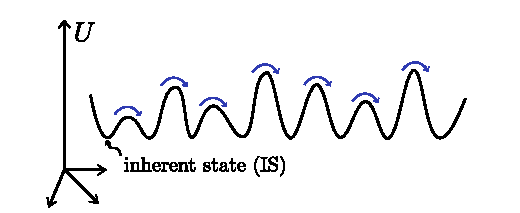
\includegraphics[width=\linewidth]{d.6-fac_results_3/pes.pdf}
\caption{Motion not only consists of hopping (excitations) but also vibrations around minima (phonons).}

\onslide<5>\centering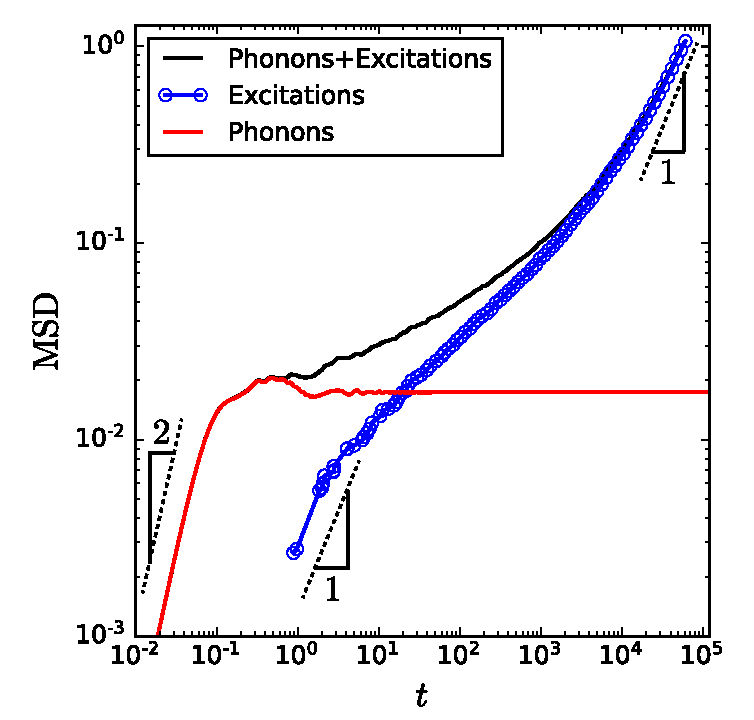
\includegraphics[valign=c,width=0.9\linewidth]{d.6-fac_results_3/newmsdphonons0.pdf}
\caption{Combining analytical formula for phonons with kMC data yields the classic MSD of supercooled liquids!}


\onslide<6>\centering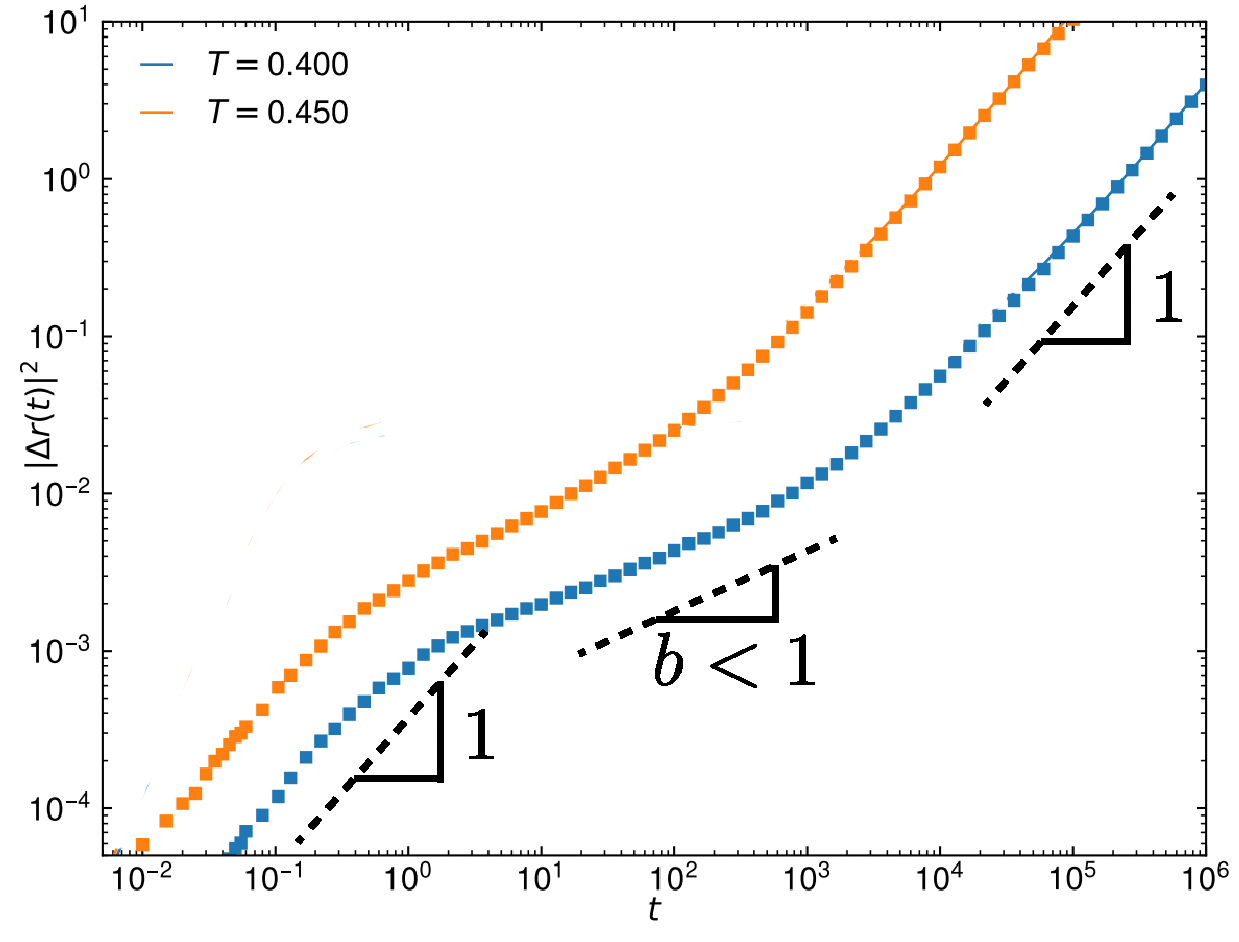
\includegraphics[valign=c,width=0.9\linewidth]{d.6-fac_results_3/ismsdmd.pdf}
\caption{The excitation part of the MSD matches with inherent structure MSD from MD simulations (Shiraishi, et al. \textit{PNAS} (2023)).}

\onslide<8->\centering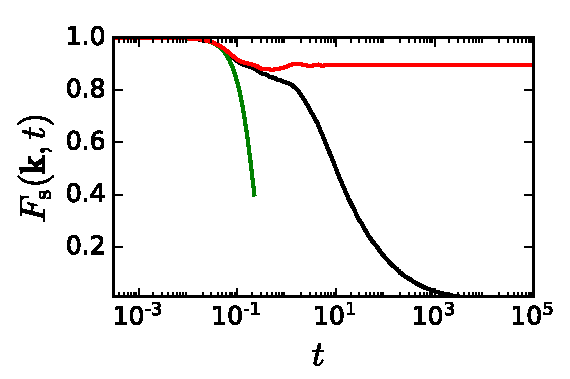
\includegraphics[valign=c,width=0.9\linewidth]{d.6-fac_results_3/newmsdphonons1.pdf}
\caption{Combining analytical formula for phonons with kMC data yields the two-stage decay in $F_\mathrm{s}(\* k,t))$. Green is the ballistic limit.}

% \onslide<6>\centering\includegraphics[valign=c,width=0.9\linewidth]{d.6-fac_results_3/fsktka.png}
% \caption{The two-stage decay in $F_\mathrm{s}(\*k,t)$ is another classic behavior!}
%\caption{Bond-order autocorrelation function $C_\mathrm{b}(t)$ at high temperatures. $\tau_\mathrm{arr} \sim e^{\beta J_\sigma}$.}    


\end{overprint}
\end{figure}

\end{column}


\begin{column}[t]{0.5\textwidth}
\vspace{-12pt}
\onslide<3->{
\begin{block}{\centering Combining Excitations and Phonons}
\centering As $T \to 0$, phonons and excitations are \textbf{uncorrelated} due to the separation of timescales.  
\end{block}
}
\begin{itemize}
    \item<4-> \textbf{Mean-Squared Displacement:} Add the contributions:
    \begin{equation*}
    \mathrm{MSD}=\mathrm{MSD}_\mathrm{ph}+\mathrm{MSD}_\mathrm{exc}
    \end{equation*}
    %\item<4-> 
    \item<7-> \textbf{Intermediate Scattering Function:} Product of the two contributions
    \begin{gather*}
    F_\mathrm{s}(\*k,t) = F^\mathrm{ph}_\mathrm{s}(\* k,t) F^\mathrm{exc}_\mathrm{s}(\* k,t)
    \\
    F^\mathrm{ph}_\mathrm{s}(\* k,t) = e^{-\frac{k^2}{4}\mathrm{MSD}^\mathrm{ph}(t)}
    \end{gather*}
    %\item<6-> The two-stage decay in $F_\mathrm{s}(\*k,t)$ is another classic behavior!
    % \item<5-> \textbf{Bond-order Autocorrelation Function:} Product of the two contributions
    % \begin{gather}
    % C_\mathrm{b}(t) = C_\mathrm{b}^\mathrm{ph}(t) C^\mathrm{exc}_\mathrm{b}(t)
    % \end{gather}
    
\end{itemize} 

\end{column}

\end{columns}

\end{frame}
